\subsection{Solar energy potential}

The Sun constantly emits a \emph{radiation flux} of around $\Phi_{\mathrm{S}} = 3,845 \cdot 10^{26} \mathrm{W}$ into space. Without any doubt it is the greatest source of renewable energy in our solar system. To determine the \emph{solar irradiance} $E_\mathrm{S}$, that arrives directly outside the Earth's atmosphere, the mean distance between the Sun and Earth $r_{\mathrm{SE}} = 149,597870 \cdot 10^{6} \mathrm{km}$ -- which is often reffered to as \emph{astronomical unit} (AU) -- needs to be taken into account as shown in equation \ref{eq:e_sun}. The result of this equation is called \emph{solar constant} \cite{Karttunen:2006, Bertol:2011, Mertens:2015, Wagner:2018}. 

\begin{center}
	\begin{equation} \label{eq:e_sun}
		E_{\mathrm{S}} = \frac{\Phi_{\mathrm{S}}}{4 \pi \, r_{\mathrm{SE}}^2} = \frac{3,845 \cdot 10^{26} \mathrm{W}}{4 \pi \cdot (1,49597870 \cdot 10^{11} \mathrm{m})^2} = 1367,21 \frac{\mathrm{W}}{\mathrm{m}^2}
	\end{equation}
\end{center}

Figure \ref{fig:tikz_angular_relationship} provides an illustration of the Sun and the Earth with consideration of the angular relationships, in which $\delta$ is the \emph{declination} of the Sun, $\varphi$ is the local \emph{latitude} of an observer on Earth and $\gamma_{\mathrm{S}}$ is the \emph{altitude} of the Sun at said latitude \cite{Appelbaum:1993, Karttunen:2006, Mertens:2015, Wagner:2018}. 

The incident rays on the hemisphere facing the Sun (separated by the dashed line in figure \ref{fig:tikz_angular_relationship}) can be assumed to be parallel to each other due to the enormous distance between the Sun and Earth \cite{Mertens:2015, Wagner:2018}.

\begin{figure}[h!]
	\centering
	

\tikzset{every picture/.style={line width=0.75pt}} %set default line width to 0.75pt        

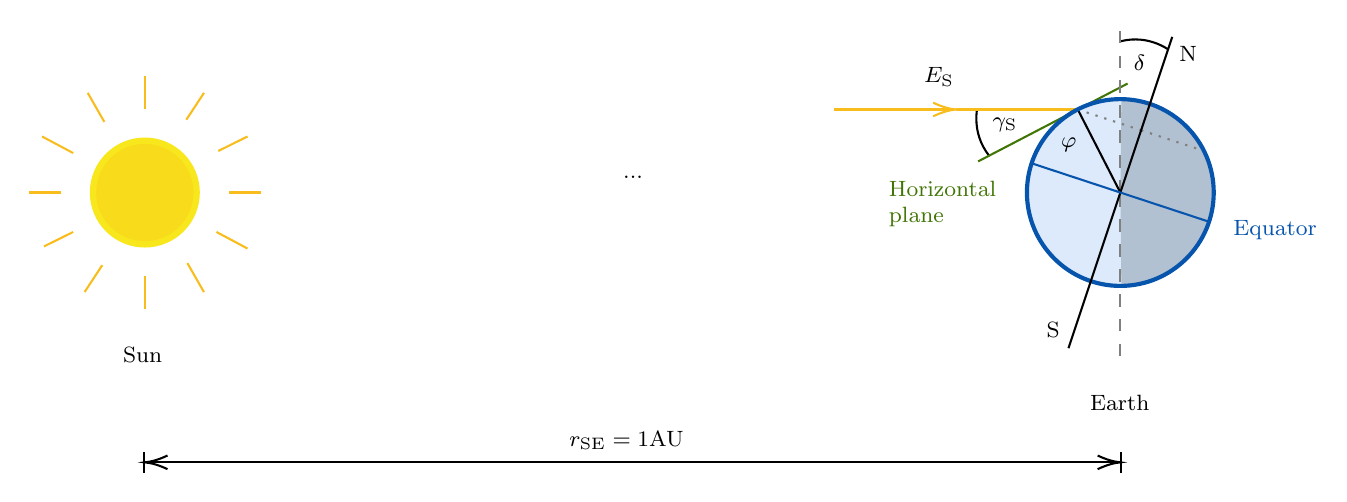
\begin{tikzpicture}[x=0.75pt,y=0.75pt,yscale=-1,xscale=1]
%uncomment if require: \path (0,447); %set diagram left start at 0, and has height of 447

%Shape: Pie [id:dp15034815819494352] 
\draw  [color={rgb, 255:red, 0; green, 0; blue, 0 }  ,draw opacity=0 ][fill={rgb, 255:red, 0; green, 0; blue, 0 }  ,fill opacity=0.45 ] (545.51,179.99) .. controls (570.29,180.26) and (590.33,200.21) .. (590.41,224.85) .. controls (590.49,249.59) and (570.42,269.74) .. (545.5,270.01) -- (545,225) -- cycle ;
%Shape: Circle [id:dp11400902817768599] 
\draw  [color={rgb, 255:red, 7; green, 84; blue, 173 }  ,draw opacity=1 ][fill={rgb, 255:red, 200; green, 222; blue, 248 }  ,fill opacity=0.64 ][line width=0.75]  (500,225) .. controls (500,200.15) and (520.15,180) .. (545,180) .. controls (569.85,180) and (590,200.15) .. (590,225) .. controls (590,249.85) and (569.85,270) .. (545,270) .. controls (520.15,270) and (500,249.85) .. (500,225) -- cycle ;
%Straight Lines [id:da48130102628083926] 
\draw [color={rgb, 255:red, 65; green, 117; blue, 5 }  ,draw opacity=1 ]   (548.5,172.5) -- (524.5,185) ;
%Shape: Arc [id:dp6322515277427461] 
\draw  [draw opacity=0] (481.9,207.42) .. controls (480.77,206.02) and (479.77,204.5) .. (478.91,202.87) .. controls (475.99,197.34) and (475.08,191.17) .. (475.92,184.97) -- (518.5,182) -- cycle ; \draw   (481.9,207.42) .. controls (480.77,206.02) and (479.77,204.5) .. (478.91,202.87) .. controls (475.99,197.34) and (475.08,191.17) .. (475.92,184.97) ;
%Straight Lines [id:da15968904032085707] 
\draw [color={rgb, 255:red, 65; green, 117; blue, 5 }  ,draw opacity=1 ]   (476.5,210) -- (524.5,185) ;
%Shape: Circle [id:dp68849801426956] 
\draw  [color={rgb, 255:red, 248; green, 231; blue, 28 }  ,draw opacity=1 ][fill={rgb, 255:red, 248; green, 220; blue, 28 }  ,fill opacity=1 ][line width=2.25]  (50,225) .. controls (50,211.19) and (61.19,200) .. (75,200) .. controls (88.81,200) and (100,211.19) .. (100,225) .. controls (100,238.81) and (88.81,250) .. (75,250) .. controls (61.19,250) and (50,238.81) .. (50,225) -- cycle ;
%Shape: Arc [id:dp11190386681659015] 
\draw  [draw opacity=0] (544.71,152.26) .. controls (547.24,151.56) and (549.86,151.21) .. (552.55,151.25) .. controls (558.14,151.31) and (563.41,153.04) .. (568.08,156.04) -- (552,196) -- cycle ; \draw   (544.71,152.26) .. controls (547.24,151.56) and (549.86,151.21) .. (552.55,151.25) .. controls (558.14,151.31) and (563.41,153.04) .. (568.08,156.04) ;
%Straight Lines [id:da09161822286264387] 
\draw [color={rgb, 255:red, 128; green, 128; blue, 128 }  ,draw opacity=1 ] [dash pattern={on 4.5pt off 4.5pt}]  (545,303.92) -- (545,225) ;
%Straight Lines [id:da48620147126216584] 
\draw [color={rgb, 255:red, 128; green, 128; blue, 128 }  ,draw opacity=1 ] [dash pattern={on 4.5pt off 4.5pt}]  (545,225) -- (545,146.08) ;
%Straight Lines [id:da2344822206483721] 
\draw [line width=0.75]    (524.5,185) -- (545,225) ;
%Straight Lines [id:da23327222270661996] 
\draw    (77,355) -- (543,355) ;
\draw [shift={(545,355)}, rotate = 180] [color={rgb, 255:red, 0; green, 0; blue, 0 }  ][line width=0.75]    (10.93,-3.29) .. controls (6.95,-1.4) and (3.31,-0.3) .. (0,0) .. controls (3.31,0.3) and (6.95,1.4) .. (10.93,3.29)   ;
\draw [shift={(75,355)}, rotate = 0] [color={rgb, 255:red, 0; green, 0; blue, 0 }  ][line width=0.75]    (10.93,-3.29) .. controls (6.95,-1.4) and (3.31,-0.3) .. (0,0) .. controls (3.31,0.3) and (6.95,1.4) .. (10.93,3.29)   ;
%Straight Lines [id:da6929947931128337] 
\draw [color={rgb, 255:red, 248; green, 189; blue, 28 }  ,draw opacity=1 ]   (407,185) -- (463.75,185) ;
\draw [shift={(465.75,185)}, rotate = 180] [color={rgb, 255:red, 248; green, 189; blue, 28 }  ,draw opacity=1 ][line width=0.75]    (10.93,-3.29) .. controls (6.95,-1.4) and (3.31,-0.3) .. (0,0) .. controls (3.31,0.3) and (6.95,1.4) .. (10.93,3.29)   ;
%Straight Lines [id:da9358361305294991] 
\draw [color={rgb, 255:red, 248; green, 189; blue, 28 }  ,draw opacity=1 ]   (524.5,185) -- (465.75,185) ;
%Straight Lines [id:da7529976931050752] 
\draw    (545.5,350) -- (545.5,360) ;
%Straight Lines [id:da4019381676598568] 
\draw [color={rgb, 255:red, 128; green, 128; blue, 128 }  ,draw opacity=1 ] [dash pattern={on 0.84pt off 2.51pt}]  (555,195) -- (585.5,205) ;
%Straight Lines [id:da051171793746800365] 
\draw [color={rgb, 255:red, 128; green, 128; blue, 128 }  ,draw opacity=1 ] [dash pattern={on 0.84pt off 2.51pt}]  (524.5,185) -- (555,195) ;
%Shape: Circle [id:dp6054942149883367] 
\draw  [color={rgb, 255:red, 7; green, 84; blue, 173 }  ,draw opacity=1 ][fill={rgb, 255:red, 200; green, 222; blue, 248 }  ,fill opacity=0 ][line width=1.5]  (500,225) .. controls (500,200.15) and (520.15,180) .. (545,180) .. controls (569.85,180) and (590,200.15) .. (590,225) .. controls (590,249.85) and (569.85,270) .. (545,270) .. controls (520.15,270) and (500,249.85) .. (500,225) -- cycle ;
%Straight Lines [id:da7513058172554794] 
\draw    (545,225) -- (520,300) ;
%Straight Lines [id:da456675238429898] 
\draw    (570,150) -- (545,225) ;
%Straight Lines [id:da7902385793672442] 
\draw [color={rgb, 255:red, 7; green, 84; blue, 173 }  ,draw opacity=1 ]   (502.5,211) -- (545,225) ;
%Straight Lines [id:da2311496114593583] 
\draw [color={rgb, 255:red, 7; green, 84; blue, 173 }  ,draw opacity=1 ]   (545,225) -- (587.5,239) ;
%Straight Lines [id:da7859324779499595] 
\draw [color={rgb, 255:red, 248; green, 189; blue, 28 }  ,draw opacity=1 ]   (75,169.06) -- (75,184.63) ;
%Straight Lines [id:da6628690922559444] 
\draw [color={rgb, 255:red, 248; green, 189; blue, 28 }  ,draw opacity=1 ]   (130.94,225) -- (115.38,225) ;
%Straight Lines [id:da059104507396427586] 
\draw [color={rgb, 255:red, 248; green, 189; blue, 28 }  ,draw opacity=1 ]   (75,280.94) -- (75,265.38) ;
%Straight Lines [id:da13924610653156622] 
\draw [color={rgb, 255:red, 248; green, 189; blue, 28 }  ,draw opacity=1 ]   (34.63,225) -- (19.06,225) ;
%Straight Lines [id:da6612538806605628] 
\draw [color={rgb, 255:red, 248; green, 189; blue, 28 }  ,draw opacity=1 ]   (109.5,244) -- (124.5,252) ;
%Straight Lines [id:da6313529241657796] 
\draw [color={rgb, 255:red, 248; green, 189; blue, 28 }  ,draw opacity=1 ]   (25.5,198) -- (40.5,206) ;
%Straight Lines [id:da5019670096718076] 
\draw [color={rgb, 255:red, 248; green, 189; blue, 28 }  ,draw opacity=1 ]   (124.5,198) -- (110.38,205) ;
%Straight Lines [id:da9267861672263464] 
\draw [color={rgb, 255:red, 248; green, 189; blue, 28 }  ,draw opacity=1 ]   (40.5,244) -- (26.38,251) ;
%Straight Lines [id:da8979247612603714] 
\draw [color={rgb, 255:red, 248; green, 189; blue, 28 }  ,draw opacity=1 ]   (95,189.94) -- (103.5,177) ;
%Straight Lines [id:da4019503947575047] 
\draw [color={rgb, 255:red, 248; green, 189; blue, 28 }  ,draw opacity=1 ]   (46,272.94) -- (54.5,260) ;
%Straight Lines [id:da27205273028090327] 
\draw [color={rgb, 255:red, 248; green, 189; blue, 28 }  ,draw opacity=1 ]   (95.5,259) -- (103.5,273) ;
%Straight Lines [id:da5079939363345163] 
\draw [color={rgb, 255:red, 248; green, 189; blue, 28 }  ,draw opacity=1 ]   (47.5,177) -- (55.5,191) ;
%Straight Lines [id:da7553342413027122] 
\draw    (74.5,360) -- (74.5,350) ;

% Text Node
\draw (515,197.4) node [anchor=north west][inner sep=0.75pt]  [font=\footnotesize]  {$\varphi $};
% Text Node
\draw (63,298) node [anchor=north west][inner sep=0.75pt]  [font=\footnotesize] [align=left] {Sun};
% Text Node
\draw (529,321) node [anchor=north west][inner sep=0.75pt]  [font=\footnotesize] [align=left] {Earth};
% Text Node
\draw (550,157.4) node [anchor=north west][inner sep=0.75pt]  [font=\footnotesize]  {$\delta $};
% Text Node
\draw (598,237) node [anchor=north west][inner sep=0.75pt]  [font=\footnotesize,color={rgb, 255:red, 7; green, 84; blue, 173 }  ,opacity=1 ] [align=left] {Equator};
% Text Node
\draw (482,187.4) node [anchor=north west][inner sep=0.75pt]  [font=\footnotesize]  {$\gamma _{\mathrm{S}}$};
% Text Node
\draw (432,218) node [anchor=north west][inner sep=0.75pt]  [font=\footnotesize,color={rgb, 255:red, 65; green, 117; blue, 5 }  ,opacity=1 ] [align=left] {Horizontal\\plane};
% Text Node
\draw (449,163.4) node [anchor=north west][inner sep=0.75pt]  [font=\footnotesize]  {$E_{\mathrm{S}}$};
% Text Node
\draw (278,338.4) node [anchor=north west][inner sep=0.75pt]  [font=\footnotesize]  {$r_{\mathrm{SE}} =1\mathrm{AU}$};
% Text Node
\draw (572,153) node [anchor=north west][inner sep=0.75pt]  [font=\footnotesize] [align=left] {N};
% Text Node
\draw (508,286) node [anchor=north west][inner sep=0.75pt]  [font=\footnotesize] [align=left] {S};
% Text Node
\draw (304,215.4) node [anchor=north west][inner sep=0.75pt]  [font=\footnotesize]  {$...$};


\end{tikzpicture}

	\caption{Angular relationship between the Sun and Earth. (Recreated from: \cite{Mertens:2015})}
	\label{fig:tikz_angular_relationship}
\end{figure} 